\chapter{Habit Features and the Switch Detector}
\label{ch:detector}

% Draft written with the phase 2 code (backend/studentide/detector/).
% Brain entries 2026-10-26-09 to -12.

\Cref{fig:detector} summarises the detector. The event log of a session is
cut into windows of $W$ seconds; each window becomes a vector of habit
features; two channels compare that vector with the student's own baseline
and feed a CUSUM change-point detector each. An alarm on either channel
marks the session for review, with an estimate of when the change happened
and which kind of change it was.

\begin{figure}[ht]
  \centering
  \resizebox{\linewidth}{!}{\tikzfig{detector}}
  \caption{The two-channel switch detector.}
  \label{fig:detector}
\end{figure}

\section{Windowing}
Windows are consecutive and non-overlapping, $W=30$\,s by default (the
window length is ablated in \cref{tab:ablation-window-length}). A window
counts only if it holds at least 20 code keystrokes; inactive windows
(reading, thinking, away) leave the detector state unchanged rather than
pulling it towards ``normal''. Keys pressed with Ctrl or Meta held,
modifiers and navigation keys are not part of the typing stream.

Keystrokes typed while the caret is inside a \texttt{\#} comment are kept
apart from code keystrokes. Lueder et al.\ observed that comment text is
typed like retyping, fluently and with few pauses \cite{lueder2026nosi}, so
mixing it in would blur the code rhythm. The comment status of each key is
recovered by replaying the edit stream (\cref{app:schema}) and checking
whether a \texttt{\#} outside a string precedes the caret on its line.
Comment keys get two features of their own, which the detector does not
use by default.

\section{Habit features}
\Cref{tab:features} lists the features. Latencies are on a log scale, so a
difference means the same for slow and fast typists. A digraph is two
consecutive code keystrokes with no deletion between them and a gap below
2\,s; longer gaps are pauses. The L-scale (second L-moment
\cite{hosking1990lmoments}) of log inter-key time is the spread measure Nosi
uses to separate composing from transcribing \cite{lueder2026nosi}.

\begin{table}[ht]
  \centering\small
  \caption{Habit features per window and the channel that uses them.}
  \label{tab:features}
  \begin{tabularx}{\linewidth}{@{}llX@{}}
    \toprule
    Group & Feature & Definition \\
    \midrule
    rhythm & \texttt{dg\_median} & median digraph latency (log ms) \\
     & \texttt{dg\_lscale} & L-scale of log inter-key time \\
     & \texttt{hold\_median} & median key hold time (log ms) \\
    digraph & \texttt{dg\_alt\_hand}, \texttt{dg\_same\_hand} & median latency when hands alternate / repeat \\
     & \texttt{dg\_to\_space}, \texttt{dg\_from\_space} & median latency into / out of the space bar \\
     & \texttt{dg\_shifted} & median latency into a shifted character \\
    \midrule
    pauses & \texttt{pause\_per\_100}, \texttt{pause\_median} & pauses ($\ge 2$\,s) per 100 keys; their median length \\
    revision & \texttt{del\_per\_100}, \texttt{del\_burst} & deletions per 100 keys; mean run of deletions \\
    build order & \texttt{nonappend\_frac}, \texttt{jump\_rate} & share of edits not at the end of the file; caret jumps $>2$ lines per minute \\
    runs & \texttt{run\_rate} & runs per minute over the trailing 5 minutes \\
    focus & \texttt{focus\_out\_rate} & window/tab focus losses per minute \\
    paste & \texttt{paste\_frac} & share of inserted characters that were pasted \\
    \midrule
    comments & \texttt{c\_dg\_median}, \texttt{c\_key\_frac} & comment digraph latency; share of keys in comments (not scored) \\
    \bottomrule
  \end{tabularx}
\end{table}

\section{Per-student baseline}
A student's baseline is fitted on their honest sessions from the first four
lab weeks and keeps only summary statistics: for every feature a robust
centre (median) and spread ($1.4826\times$ MAD, with a small floor so that a
habit the student never varies, such as pasting, does not explode), plus the
mean $\mu_0$ and standard deviation $\sigma_0$ of the student's own distance
score. $\mu_0$ and $\sigma_0$ are estimated leave-one-session-out, so they
describe a \emph{new} honest session rather than the sessions the centre was
fitted on. Nothing else is stored, which lets the raw baseline keystrokes be
deleted as promised on the consent screen.

\section{Distance score and the two channels}
For window $t$ and feature $f$, $z_{tf}=|x_{tf}-c_f|/s_f$, clipped at 6.
The distance is a weighted root mean square,
\begin{equation}
  d_t=\sqrt{\frac{\sum_f w_f z_{tf}^2}{\sum_f w_f}},\qquad
  x_t=\frac{d_t-\mu_0}{\sigma_0}.
\end{equation}

A single score over all features turned out to be a poor compromise
(\cref{tab:ablation-feature-groups}): equal weights let the many noisy
process features drown the typing rhythm, and weighting by how well a
feature separates students drowns the process features that reveal copying
and pasting. The detector therefore runs two channels:
\begin{description}
  \item[Identity] (rhythm and digraph groups) asks whether the same hands
  are typing. Weights $w_f$ are the intraclass correlation of the feature
  across students' baseline windows \cite{shrout1979icc}, between-student
  variance over total variance. They need only honest baseline data from all
  students, no impostor examples.
  \item[Process] (pauses, revisions, build order, runs, focus, paste), equal
  weights, asks whether the way of working changed. It catches copying out
  and pasting by the student themselves, which the identity channel cannot
  see.
\end{description}

\section{CUSUM change-point detection}
Each channel runs a one-sided CUSUM \cite{page1954continuous,basseville1993detection}
on its standardised score,
\begin{equation}
  S_t=\max(0,\,S_{t-1}+x_t-k),
\end{equation}
skipping inactive windows. An alarm is raised when $S_t>h$, and the switch
time is estimated as the start of the window after the last $t$ with
$S_t=0$. After an alarm $S$ restarts at zero, so every false alarm in a long
honest session is counted. The identity channel uses $k=1$ (a typist change
moves its score by several $\sigma_0$, and the larger $k$ absorbs
day-to-day drift), the process channel $k=0.5$. The threshold $h$ of each
channel is set on calibration students so that the two channels together
give at most 0.2 false alarms per hour of honest work.
\Cref{fig:cusum-trace} shows a takeover being caught.

\begin{figure}[ht]
  \centering
  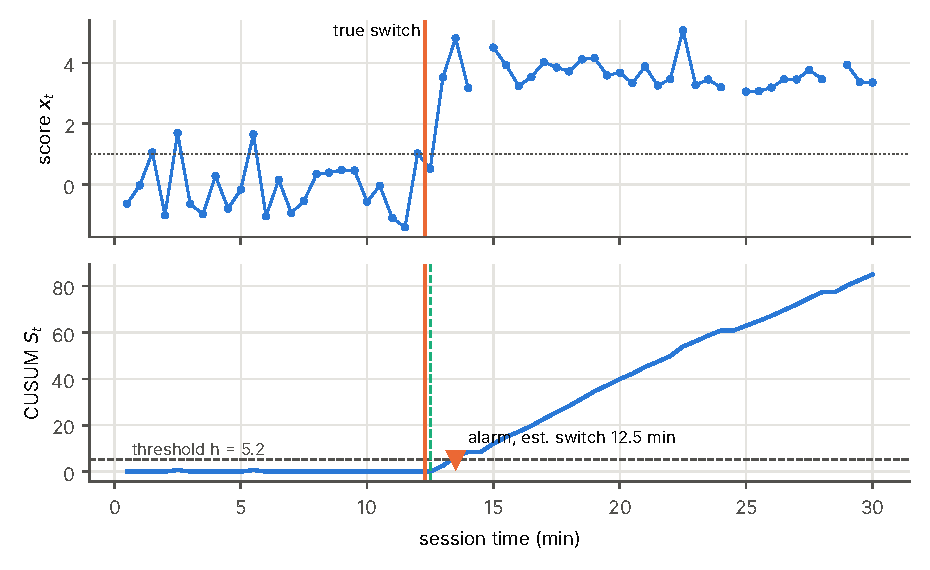
\includegraphics[width=0.85\linewidth]{cusum-trace-takeover}
  \caption{Identity channel on a synthetic session in which a speed-matched
    partner takes over. Top: standardised score per 30\,s window (gaps are
    inactive windows; dotted line $k$). Bottom: CUSUM statistic, threshold
    $h$, alarm and estimated switch time.}
  \label{fig:cusum-trace}
\end{figure}

\section{Baselines}
Scaled Manhattan \cite{killourhy2009comparing}, TypeNet-style
\cite{acien2022typenet}, Nosi IAT rhythm \cite{lueder2026nosi}. A Nosi-style
detector (the L-scale feature alone, same CUSUM) is already part of the
ablation; the other two are planned for the evaluation harness (phase 4).

\section{Synthetic-data pipeline}
Before Phase 2 data exists, the detector is built and tuned on simulated
sessions written in the editor's own event format, so the same code reads
simulated and real logs (\cref{fig:synthetic-evaluation}). Each simulated
typist has a stable habit profile: base digraph latency and spread,
personal digraph offsets, a hand-alternation speed-up, hold time, word-level
hesitations and think pauses before lines, typo and revision rates,
skeleton-first or linear code order, run frequency and how often they look
away. Every session adds day-to-day drift to each habit. The typists write
lab-style Python programs (with comments) until the session ends.

The five study conditions are simulated as: (A) honest composing; (B) a
different typist composes the whole session; (C) a second typist takes over
at a random minute after a 5--40\,s seat swap and continues the same code;
(D) the student switches to transcribing code from elsewhere (faster, more
uniform rhythm, fewer pauses and typos, glances away every 12--40
characters); (E) the student pastes chunks copied from elsewhere. Partners
for B and C are the typist nearest in base speed, a stand-in for the
study's grade-matched proxies; C is also run with a random partner.

\begin{figure}[ht]
  \centering
  \resizebox{\linewidth}{!}{\tikzfig{synthetic-evaluation}}
  \caption{Synthetic evaluation protocol.}
  \label{fig:synthetic-evaluation}
\end{figure}

Known simplifications: indentation is typed with Tab whereas the real
editor auto-indents and auto-closes brackets, mouse-driven editing is not
simulated, and simulated habits are independent draws, so real students
will be both more alike (shared curriculum, same keyboards) and more
variable (fatigue, difficulty of the task). The synthetic numbers show that
the pipeline works and how its settings trade off; they are not a claim
about real students.
